\documentclass{article}

\PassOptionsToPackage{numbers, compress}{natbib}
\usepackage[dblblindworkshop]{neurips_2026}
\workshoptitle{Attributing Model Behavior at Scale: Data Attribution and Provenance (ATTRIB 2026)}

\usepackage[utf8]{inputenc}
\usepackage[T1]{fontenc}
\usepackage{hyperref}
\usepackage{url}
\usepackage{booktabs}
\usepackage{amsfonts}
\usepackage{amsmath}
\usepackage{nicefrac}
\usepackage{microtype}
\usepackage{xcolor}
\usepackage{multirow}
\usepackage{graphicx}

\title{Mechanistic Attribution of Relational Transformer Behavior to Synthetic Pretraining Generators}

\author{%
  Anonymous Author(s) \\
  Affiliation \\
  \texttt{email@domain.com}
}

\begin{document}

\maketitle

\begin{abstract}
When a relational foundation model (RFM) is pretrained on synthetic relational databases, benchmark comparisons tell us \emph{which} generator produced a better model but not \emph{why}, or whether the advantage reflects a genuine relational skill rather than better marginal statistics. We treat this as a mechanistic data-attribution problem: given four Relational Transformer (RT) checkpoints that share architecture, initialization, and step budget and differ only in the synthetic-data generator that produced their pretraining corpus (RelDiff, GRDM, PluRel, RDB-PFN), we trace the generator's fingerprint from weight space, through learned representations and attention structure, to the model's downstream benchmark behavior. Weight-space divergence, representational similarity (CKA), and within-neighborhood attention entropy all agree on the same ranking: only the generator whose synthetic construction makes relational structure necessary for reconstructing masked values (RelDiff) yields a model that mechanistically relies on cross-table structure out of distribution. We then close the loop causally: intervening on exactly the mechanism identified by these diagnostics --- corrupting foreign-key structure or zeroing the cross-table attention stream at inference --- reproduces the model's downstream degradation quantitatively, including on the specific tasks and context lengths where the mechanism predicts an effect and where it does not. This provides a template for attributing foundation-model capabilities to specific, checkable properties of a synthetic pretraining corpus, rather than to the generator's identity alone.
\end{abstract}

\section{Introduction}
\label{sec:intro}

A growing family of relational foundation models (RFMs) --- Griffin \cite{griffin}, KumoRFM \cite{kumorfm}, and the Relational Transformer (RT) \cite{rt} among them --- are pretrained on large corpora of synthetic relational databases rather than on a single fixed dataset, because real multi-table databases \cite{rdl,relbench} with the necessary scale and diversity are scarce and often proprietary. This creates a data-attribution problem that is one step removed from the usual training-example-level setting studied at this workshop: the object whose contribution we want to attribute is not a training example but a \emph{generator} --- a procedure that induces a distribution over synthetic databases. Downstream benchmarks can rank generators, but a benchmark ranking is a black-box comparison: it does not say what property of a generator's output caused the ranking, whether the advantage will transfer to schemas unlike anything the generator produced, or whether the model actually learned to \emph{use} relational structure versus merely fitting the generator's marginal statistics. Because the pretraining objective is masked-cell reconstruction, this last question is exactly the ambiguity mechanistic interpretability is suited to resolve: a well-fit marginal distribution and a genuine relational computation both lower reconstruction loss, but only one of them is a transferable skill.

We study this question in the cleanest setting available: four RT checkpoints, byte-identical in architecture (12 blocks, $d{=}256$, 19.2M parameters, three attention streams per block), initialization, and step budget, pretrained on corpora from four synthetic relational-database generators representing distinct design philosophies --- two condition on real reference databases (RelDiff: joint multi-hop graph diffusion; GRDM: graph-conditional diffusion with 1-hop locality) and two synthesize schemas and values from scratch with no reference data (PluRel, RDB-PFN). Because the only experimental variable across the four arms is the generator, any measured difference between the four checkpoints is attributable to the data it produced, not to confounds of architecture or optimization.

\textbf{Contributions.} (1) We measure, in the corpora themselves and with no model involved, how much of a masked cell's recoverable signal lives in neighbouring tables (Sec.~\ref{sec:corpus}); this turns the property our account rests on into a measured quantity that already orders the generators. (2) We give a weight-space and representational diagnostic (Sec.~\ref{sec:mech}) that predicts, from a checkpoint alone, whether a generator taught the model to treat cross-table structure as predictive or to pool over it. (3) We show this diagnostic is causally load-bearing, not merely correlational (Sec.~\ref{sec:bridge}): ablating the identified mechanism at inference reproduces the corresponding benchmark degradation, including a case where the mechanism's own failure mode --- misleading structural priors on one schema --- correctly predicts a benchmark loss rather than a gain. Together these give a recipe for attributing what a synthetic-data generator teaches a foundation model beyond a single benchmark number.

\section{Setup: a controlled comparison across four generators}
\label{sec:setup}

\textbf{Generators.} The four generators span the two structurally distinct families of reference-free vs.\ reference-conditioned synthesis. \emph{RelDiff} \cite{reldiff} and \emph{GRDM} \cite{grdm} copy a real reference database's schema and foreign-key (FK) graph and regenerate attributes with a diffusion model, jointly (RelDiff, multi-hop) or locally (GRDM, 1-hop, non-diffusion in-degree sampling for structure). \emph{PluRel} \cite{plurel} and \emph{RDB-PFN} \cite{rdbpfn} require no reference: they sample a schema and PK--FK graph from a hand-designed prior and generate attribute values with structural causal models. Each arm was pretrained on a corpus of 1{,}000 generated databases. None of the four learns a schema prior from data --- schema is either copied verbatim or hand-designed --- so any difference in downstream relational behavior must come from how each generator couples attribute values to graph structure, not from schema diversity per se.

\textbf{Models.} Each of the four RT checkpoints (\texttt{reldiff\_final.pt}, \texttt{grdm\_final.pt}, \texttt{plurel\_final.pt}, \texttt{rdbpfn\_final.pt}) was pretrained with the identical masked-value-reconstruction objective, encoder set (typed value encoders for number/text/datetime/boolean, 384-d MiniLM \cite{minilm} text embeddings), and step budget, from a shared initialization. The shared initialization is verifiable from the checkpoints rather than assumed: 132 tensors (115{,}585 parameters, chiefly decoder heads and type norms) are \emph{bitwise} identical across all four arms, which independently trained models cannot achieve by coincidence. The RT architecture separates attention into three interpretable streams per block: \texttt{col} (column-level), \texttt{feat} (row/feature-level, which includes a cell's parent rows via \texttt{kv\_in\_f2p}), and \texttt{nbr} (neighbor attention, architecturally masked to FK-linked cells). Both cross-table routes are built from the same \texttt{f2p\_nbr\_idxs} tensor, and intervening on each separately shows they operate \emph{in series} rather than in parallel: \texttt{nbr} lets a parent aggregate its children, but that aggregate reaches a masked cell only through \texttt{feat}'s parent-cell inclusion. Blocking the \texttt{feat} route costs RelDiff $+0.193$ masked-cell loss and additionally zeroing \texttt{nbr} costs nothing further ($+0.193$, identical), while zeroing \texttt{nbr} alone costs $+0.132$. The \texttt{feat} path is therefore the bottleneck through which cross-table information must pass, and \texttt{nbr} feeds it rather than substituting for it. This separation is what makes the checkpoints diagnosable: a generator's imprint on \emph{relational} computation and its imprint on \emph{marginal/attribute} statistics land in different, nameable parts of the network.

\textbf{Evaluation.} All mechanistic probes (Sec.~\ref{sec:mech}) use three RelBench databases (\texttt{rel-ratebeer}, \texttt{rel-arxiv}, \texttt{rel-stack}) that lie outside every generator's pretraining reference set, so results reflect out-of-distribution transfer rather than memorization of a shared reference. The downstream benchmark (Sec.~\ref{sec:bridge}) covers 9 RelBench tasks across 5 in-context lengths (100--30{,}000 tokens), the same in-context-learning protocol used to compare the checkpoints as generative pretrained models.

% Drop-in section for the E2 corpus measurement.
% To include: put % Drop-in section for the E2 corpus measurement.
% To include: put % Drop-in section for the E2 corpus measurement.
% To include: put \input{section_e2} immediately before \section{Mechanistic fingerprint...}
% Costs roughly half a page. Frees space by trimming Related Work (Sec. 6) and the
% second paragraph of Sec. 3's "Behavioral reliance" discussion.

\section{What the corpora make predictable}
\label{sec:corpus}

The account above rests on \emph{predictive necessity}: because the pretraining objective is
masked-cell reconstruction, a corpus can only teach cross-table computation if its masked cells
are hard to recover from their own row. That is a property of the data, not of any model, so we
measure it directly and without involving the RT at all.

For each corpus we sample 40 databases, recover the FK graph, and for each target column fit
identical gradient-boosted regressors three times: from the target's own row; from its own row
plus the columns of its FK parents; and from its own row plus aggregates over its FK children.
The gain from adding relational features is the neighbour predictive information in that corpus.
Splitting parents from children matters because the two map onto different routes in the RT: a
cell reading its parents flows through the \texttt{feat} stream's parent-cell inclusion, while
aggregation over children is what the \texttt{nbr} stream does. Scores are clipped to $[-1,1]$
before differencing, since unbounded negative $R^2$ lets one diverged fit dominate a mean, and we
report medians with 95\% bootstrap intervals.

\begin{table}[t]
\caption{Neighbour predictive information per corpus, measured with no RT involved (40 databases
each; median, 95\% bootstrap CI). RelDiff is the only corpus in which reading a neighbouring table
measurably helps recover a held-out cell. RDB-PFN is its mirror image: the most learnable
within-row structure of any corpus and no relational signal at all.}
\label{tab:e2}
\centering
\small
\begin{tabular}{lcccc}
\toprule
Corpus & Tasks & Own-row $R^2$ & Parent lift & Child lift \\
\midrule
RelDiff & 48  & 0.022 & \textbf{+0.072 [+0.018, +0.091]} & $-$0.001 \\
PluRel  & 113 & 0.166 & +0.009 [+0.001, +0.022] & $-$0.000 \\
RDB-PFN & 120 & 0.436 & +0.001 [$-$0.004, +0.009] & $-$0.005 \\
GRDM    & 120 & $-$0.011 & $-$0.057 [$-$0.076, $-$0.044] & $-$0.105 \\
\bottomrule
\end{tabular}
\end{table}

Table~\ref{tab:e2} orders the generators the same way every downstream measurement does, and it
does so before any model is trained. RelDiff's parent lift is eight times PluRel's and roughly
seventy times RDB-PFN's, whose interval spans zero. Read as a share of the predictable signal,
neighbours contribute 77\% for RelDiff, 5\% for PluRel and 0.1\% for RDB-PFN. RelDiff's cells are
close to unrecoverable from their own row ($R^2$ 0.022) and become recoverable once a parent is
visible, which is precisely the condition under which masked-cell reconstruction rewards learning
to read across tables. RDB-PFN's profile --- the most predictable rows and no relational signal
--- is the data-side counterpart of its benchmark behaviour, strong at short context and untouched
by ablation.

Two qualifications. Child lift is flat in every corpus, RelDiff included, so what its data
rewards specifically is reading parents; the transfer to child-aggregation tasks at benchmark time
is not something the corpus directly incentivises, and our aggregates (mean, standard deviation,
count) may simply be too coarse to capture it. Second, GRDM's negative lift is best read alongside
a property of its shipped corpus rather than its design: every string and datetime column was
converted to a float and never converted back, so its databases carry no text or categorical
columns at all (0 against RelDiff's 234 over the same references). The RT's text encoder and
MiniLM pathway therefore received no signal in that arm, which is a confound worth stating
plainly: the GRDM arm differs from the others in more than its generator.

\paragraph{Diversity is not the mechanism.}
A natural alternative is that RelDiff simply produces more diverse data. Measuring feature, table
and cross-table diversity directly from the generated databases --- never through any of the four
models, so the measurement cannot be an artifact of what it explains --- RelDiff is indeed most
diverse on all three axes (1.10 / 0.57 / 1.04). But the ranking of the others does not track
mechanism formation: PluRel exceeds GRDM on cross-table diversity (0.85 vs.\ 0.71) yet learns no
usable relational computation (Table~\ref{tab:e7}), while GRDM does on in-distribution schemas.
Diversity describes a generator's marginal output; predictive necessity describes whether values
are \emph{coupled} to structure, and only the latter separates the four models.
 immediately before \section{Mechanistic fingerprint...}
% Costs roughly half a page. Frees space by trimming Related Work (Sec. 6) and the
% second paragraph of Sec. 3's "Behavioral reliance" discussion.

\section{What the corpora make predictable}
\label{sec:corpus}

The account above rests on \emph{predictive necessity}: because the pretraining objective is
masked-cell reconstruction, a corpus can only teach cross-table computation if its masked cells
are hard to recover from their own row. That is a property of the data, not of any model, so we
measure it directly and without involving the RT at all.

For each corpus we sample 40 databases, recover the FK graph, and for each target column fit
identical gradient-boosted regressors three times: from the target's own row; from its own row
plus the columns of its FK parents; and from its own row plus aggregates over its FK children.
The gain from adding relational features is the neighbour predictive information in that corpus.
Splitting parents from children matters because the two map onto different routes in the RT: a
cell reading its parents flows through the \texttt{feat} stream's parent-cell inclusion, while
aggregation over children is what the \texttt{nbr} stream does. Scores are clipped to $[-1,1]$
before differencing, since unbounded negative $R^2$ lets one diverged fit dominate a mean, and we
report medians with 95\% bootstrap intervals.

\begin{table}[t]
\caption{Neighbour predictive information per corpus, measured with no RT involved (40 databases
each; median, 95\% bootstrap CI). RelDiff is the only corpus in which reading a neighbouring table
measurably helps recover a held-out cell. RDB-PFN is its mirror image: the most learnable
within-row structure of any corpus and no relational signal at all.}
\label{tab:e2}
\centering
\small
\begin{tabular}{lcccc}
\toprule
Corpus & Tasks & Own-row $R^2$ & Parent lift & Child lift \\
\midrule
RelDiff & 48  & 0.022 & \textbf{+0.072 [+0.018, +0.091]} & $-$0.001 \\
PluRel  & 113 & 0.166 & +0.009 [+0.001, +0.022] & $-$0.000 \\
RDB-PFN & 120 & 0.436 & +0.001 [$-$0.004, +0.009] & $-$0.005 \\
GRDM    & 120 & $-$0.011 & $-$0.057 [$-$0.076, $-$0.044] & $-$0.105 \\
\bottomrule
\end{tabular}
\end{table}

Table~\ref{tab:e2} orders the generators the same way every downstream measurement does, and it
does so before any model is trained. RelDiff's parent lift is eight times PluRel's and roughly
seventy times RDB-PFN's, whose interval spans zero. Read as a share of the predictable signal,
neighbours contribute 77\% for RelDiff, 5\% for PluRel and 0.1\% for RDB-PFN. RelDiff's cells are
close to unrecoverable from their own row ($R^2$ 0.022) and become recoverable once a parent is
visible, which is precisely the condition under which masked-cell reconstruction rewards learning
to read across tables. RDB-PFN's profile --- the most predictable rows and no relational signal
--- is the data-side counterpart of its benchmark behaviour, strong at short context and untouched
by ablation.

Two qualifications. Child lift is flat in every corpus, RelDiff included, so what its data
rewards specifically is reading parents; the transfer to child-aggregation tasks at benchmark time
is not something the corpus directly incentivises, and our aggregates (mean, standard deviation,
count) may simply be too coarse to capture it. Second, GRDM's negative lift is best read alongside
a property of its shipped corpus rather than its design: every string and datetime column was
converted to a float and never converted back, so its databases carry no text or categorical
columns at all (0 against RelDiff's 234 over the same references). The RT's text encoder and
MiniLM pathway therefore received no signal in that arm, which is a confound worth stating
plainly: the GRDM arm differs from the others in more than its generator.

\paragraph{Diversity is not the mechanism.}
A natural alternative is that RelDiff simply produces more diverse data. Measuring feature, table
and cross-table diversity directly from the generated databases --- never through any of the four
models, so the measurement cannot be an artifact of what it explains --- RelDiff is indeed most
diverse on all three axes (1.10 / 0.57 / 1.04). But the ranking of the others does not track
mechanism formation: PluRel exceeds GRDM on cross-table diversity (0.85 vs.\ 0.71) yet learns no
usable relational computation (Table~\ref{tab:e7}), while GRDM does on in-distribution schemas.
Diversity describes a generator's marginal output; predictive necessity describes whether values
are \emph{coupled} to structure, and only the latter separates the four models.
 immediately before \section{Mechanistic fingerprint...}
% Costs roughly half a page. Frees space by trimming Related Work (Sec. 6) and the
% second paragraph of Sec. 3's "Behavioral reliance" discussion.

\section{What the corpora make predictable}
\label{sec:corpus}

The account above rests on \emph{predictive necessity}: because the pretraining objective is
masked-cell reconstruction, a corpus can only teach cross-table computation if its masked cells
are hard to recover from their own row. That is a property of the data, not of any model, so we
measure it directly and without involving the RT at all.

For each corpus we sample 40 databases, recover the FK graph, and for each target column fit
identical gradient-boosted regressors three times: from the target's own row; from its own row
plus the columns of its FK parents; and from its own row plus aggregates over its FK children.
The gain from adding relational features is the neighbour predictive information in that corpus.
Splitting parents from children matters because the two map onto different routes in the RT: a
cell reading its parents flows through the \texttt{feat} stream's parent-cell inclusion, while
aggregation over children is what the \texttt{nbr} stream does. Scores are clipped to $[-1,1]$
before differencing, since unbounded negative $R^2$ lets one diverged fit dominate a mean, and we
report medians with 95\% bootstrap intervals.

\begin{table}[t]
\caption{Neighbour predictive information per corpus, measured with no RT involved (40 databases
each; median, 95\% bootstrap CI). RelDiff is the only corpus in which reading a neighbouring table
measurably helps recover a held-out cell. RDB-PFN is its mirror image: the most learnable
within-row structure of any corpus and no relational signal at all.}
\label{tab:e2}
\centering
\small
\begin{tabular}{lcccc}
\toprule
Corpus & Tasks & Own-row $R^2$ & Parent lift & Child lift \\
\midrule
RelDiff & 48  & 0.022 & \textbf{+0.072 [+0.018, +0.091]} & $-$0.001 \\
PluRel  & 113 & 0.166 & +0.009 [+0.001, +0.022] & $-$0.000 \\
RDB-PFN & 120 & 0.436 & +0.001 [$-$0.004, +0.009] & $-$0.005 \\
GRDM    & 120 & $-$0.011 & $-$0.057 [$-$0.076, $-$0.044] & $-$0.105 \\
\bottomrule
\end{tabular}
\end{table}

Table~\ref{tab:e2} orders the generators the same way every downstream measurement does, and it
does so before any model is trained. RelDiff's parent lift is eight times PluRel's and roughly
seventy times RDB-PFN's, whose interval spans zero. Read as a share of the predictable signal,
neighbours contribute 77\% for RelDiff, 5\% for PluRel and 0.1\% for RDB-PFN. RelDiff's cells are
close to unrecoverable from their own row ($R^2$ 0.022) and become recoverable once a parent is
visible, which is precisely the condition under which masked-cell reconstruction rewards learning
to read across tables. RDB-PFN's profile --- the most predictable rows and no relational signal
--- is the data-side counterpart of its benchmark behaviour, strong at short context and untouched
by ablation.

Two qualifications. Child lift is flat in every corpus, RelDiff included, so what its data
rewards specifically is reading parents; the transfer to child-aggregation tasks at benchmark time
is not something the corpus directly incentivises, and our aggregates (mean, standard deviation,
count) may simply be too coarse to capture it. Second, GRDM's negative lift is best read alongside
a property of its shipped corpus rather than its design: every string and datetime column was
converted to a float and never converted back, so its databases carry no text or categorical
columns at all (0 against RelDiff's 234 over the same references). The RT's text encoder and
MiniLM pathway therefore received no signal in that arm, which is a confound worth stating
plainly: the GRDM arm differs from the others in more than its generator.

\paragraph{Diversity is not the mechanism.}
A natural alternative is that RelDiff simply produces more diverse data. Measuring feature, table
and cross-table diversity directly from the generated databases --- never through any of the four
models, so the measurement cannot be an artifact of what it explains --- RelDiff is indeed most
diverse on all three axes (1.10 / 0.57 / 1.04). But the ranking of the others does not track
mechanism formation: PluRel exceeds GRDM on cross-table diversity (0.85 vs.\ 0.71) yet learns no
usable relational computation (Table~\ref{tab:e7}), while GRDM does on in-distribution schemas.
Diversity describes a generator's marginal output; predictive necessity describes whether values
are \emph{coupled} to structure, and only the latter separates the four models.


\section{Mechanistic fingerprint: weight space, function, and attention}
\label{sec:mech}

\textbf{Weight space (E1).} Because all four arms share an initialization, we measure each checkpoint's deviation from the 4-model mean, grouped by stream and by depth. Table~\ref{tab:e1} shows the deviation norm for each attention stream. RelDiff is the only arm whose largest deviation is in \texttt{nbr}-attention (6.43, vs.\ 3.8--5.6 for the other three, where \texttt{nbr} is always the \emph{smallest} deviating stream); GRDM's largest deviation is in \texttt{feat}-attention (7.18). PluRel and RDB-PFN move least overall and in a shared direction (pairwise deviation cosine $+0.11$, against a $-1/3$ baseline for unrelated directions). This is a purely weight-based signature, available in minutes on a CPU without any dataloader, and it predicts the functional and behavioral results below \emph{before} they were measured.

\begin{table}[t]
\caption{E1: per-stream weight deviation from the 4-model mean (L2 norm; larger = more specialized by that stream). RelDiff uniquely peaks in \texttt{nbr}; GRDM peaks in \texttt{feat}; PluRel/RDB-PFN are near-identical and diffuse.}
\label{tab:e1}
\centering
\small
\begin{tabular}{lccccc}
\toprule
Model & Encoders & Col-attn & Feat-attn & Nbr-attn & FFN \\
\midrule
GRDM     & 1.95 & 6.10 & \textbf{7.18} & 5.55 & 10.82 \\
PluRel   & 1.05 & 5.13 & 4.68 & 3.90 & 7.69 \\
RDB-PFN  & 1.03 & 5.57 & 4.35 & 3.80 & 7.51 \\
RelDiff  & 1.64 & 5.37 & 5.88 & \textbf{6.43} & 9.49 \\
\bottomrule
\end{tabular}
\end{table}

\textbf{Function (E4).} Weight distance can overstate differences if different weights compute the same function, so we also measure linear CKA between residual-stream activations on identical real-data batches (Table~\ref{tab:e4cka}, left/right = early/late blocks). Functional divergence grows monotonically with depth for every pair: all four models agree on early featurization (CKA $\geq 0.80$ in blocks 0--5) and diverge in late relational integration. Notably, function and weights disagree on which models cluster: GRDM and RelDiff --- weight-space outliers in Table~\ref{tab:e1} --- are the most functionally \emph{similar} pair late (0.824), while RDB-PFN, PluRel's weight-space twin, is the functional outlier (as low as 0.406 against GRDM). Weight direction measures what a corpus pushed on; CKA measures where the computation landed on real inputs; both are needed because they can disagree.

\begin{table}[t]
\caption{E4 (CKA, real data) and E5 (within-FK-neighborhood attention). Real-reference generators (RelDiff, GRDM) produce the most functionally divergent-yet-mutually-similar late representations and the sharpest (lowest-entropy) attention within the FK neighborhood; PluRel/RDB-PFN pool near-uniformly.}
\label{tab:e4cka}
\centering
\small
\begin{tabular}{lcc|lcc}
\toprule
\multicolumn{3}{c|}{E4: CKA (early / late blocks)} & \multicolumn{3}{c}{E5: attention within FK neighborhood} \\
Pair & Early & Late & Model & Norm. entropy & Top-1 mass \\
\midrule
GRDM$\sim$RelDiff  & 0.944 & \textbf{0.824} & RelDiff & \textbf{0.843} & \textbf{0.396} \\
PluRel$\sim$RelDiff& 0.944 & 0.810          & GRDM    & 0.858 & 0.394 \\
GRDM$\sim$PluRel   & 0.938 & 0.718          & RDB-PFN & 0.890 & 0.361 \\
PluRel$\sim$RDB-PFN& 0.909 & 0.707          & PluRel  & 0.898 & 0.361 \\
RDB-PFN$\sim$RelDiff&0.870 & 0.587          & & & \\
GRDM$\sim$RDB-PFN  & 0.808 & \textbf{0.406} & & & \\
\bottomrule
\end{tabular}
\end{table}

\textbf{Attention (E5).} The RT's \texttt{nbr} attention is architecturally masked to FK-linked cells ($\leq 5$ edges/row), so whether heads can attend across tables is fixed by construction; what a generator can teach is \emph{how attention is distributed within} that permitted neighborhood. We hook \texttt{wq}/\texttt{wk} inputs and recompute masked softmax scores on fixed probe batches. Table~\ref{tab:e4cka} (right) shows RelDiff and GRDM --- the two real-reference generators --- produce measurably sharper (lower-entropy) within-neighborhood attention than PluRel and RDB-PFN, which are close to uniform. Selection versus pooling is exactly the operation that should behave differently as context grows: pooling dilutes with more neighbors, selection does not.

\textbf{Behavioral reliance (E7).} Attention structure shows what information \emph{could} be used; we test what is \emph{actually used} with input corruptions on real held-out data: intact inputs, FK links shuffled within a table (structure destroyed, marginals intact), and neighbors dropped. We define a structure-reliance index as the reconstruction-loss increase under FK shuffling, and separately measure the loss increase from zeroing the \texttt{nbr} stream at inference. Table~\ref{tab:e7} shows RelDiff is the only model with non-trivial reliance on either intervention (+20\% loss under FK shuffling); the other three are within $\pm2\%$ of intact loss under every corruption, i.e., functionally indifferent to relational structure on unseen schemas, despite GRDM's sharp attention in Table~\ref{tab:e4cka}. Blanking the FK links rather than shuffling them reproduces the same pattern (RelDiff $+0.065$, all others $\leq 0.014$), so the effect is not an artifact of the particular corruption used. Two controls sharpen this. Corrupting a graded fraction of FK links rather than all of them yields a monotone loss curve for RelDiff and near-flat lines for the rest, with RelDiff's slope $11$--$29\times$ the others'. And an \emph{untrained} RT, scored identically, already degrades $4.9\%$ under FK shuffling, simply because altering the mask alters the computation. Against that floor the three structure-blind arms sit at $0.7$--$1.3\times$ --- statistically indistinguishable from a network that never trained --- while RelDiff reaches $17\times$. Their indifference is therefore not a small effect but the absence of one.\footnote{The graded and untrained-floor controls were run on \texttt{rel-stack} alone rather than the full three-database probe suite, so their absolute losses are not comparable to the table; the ratios are what we report.} GRDM's relational knowledge is schema-\emph{specific}: it learned regularities of its own reference databases rather than a transferable use of FK structure.

\begin{table}[t]
\caption{E7: masked-reconstruction loss under corruption (mean over 3 held-out real DBs, 27 probe batches). RelDiff is the only model that degrades under structural corruption; all others are within noise.}
\label{tab:e7}
\centering
\small
\begin{tabular}{lcccc}
\toprule
Model & Intact loss & $\Delta$ nbr zeroed & $\Delta$ FK shuffled & $\Delta$ FK blanked \\
\midrule
RelDiff  & \textbf{0.339} & \textbf{+0.029} & \textbf{+0.069 (+20\%)} & +0.065 \\
PluRel   & 0.339 & +0.007 & +0.009 & +0.014 \\
GRDM     & 0.350 & +0.013 & $-$0.005 & $-$0.007 \\
RDB-PFN  & 0.351 & $-$0.002 & +0.003 & +0.007 \\
\bottomrule
\end{tabular}
\end{table}

The three diagnostics agree: RelDiff's corpus is the only one that makes cross-table structure predictively necessary for reconstruction, and that is the only corpus whose model both attends selectively within the FK neighborhood and functionally relies on it out of distribution. This is consistent with the underlying generative process --- RelDiff regenerates attributes \emph{conditioned on} neighboring tables via joint multi-hop diffusion, so a masked value's neighbors genuinely carry information about it, and training pressure lands on the \texttt{nbr} stream (E1) before we ever measure function or behavior.

\section{Closing the loop: does the mechanism cause the benchmark result?}
\label{sec:bridge}

Sec.~\ref{sec:mech} establishes a correlational story: the generator that induces relational reliance also produces the model with the best downstream benchmark profile (mean AUROC over the six classification tasks at context 1024: RelDiff 0.748 $>$ RDB-PFN 0.740 $>$ PluRel 0.723 $>$ GRDM 0.666), and RelDiff degrades least as context grows from 1024 to 30{,}000 tokens. This comparison needed care, because the two tasks that drive it are rare-label ones (\texttt{rel-stack} user-engagement and user-badge) that at our original $n{=}256$ contributed only six and ten positive examples, enough for a Hanley--McNeil interval \cite{hanley} of $\pm 0.073$. We therefore rescored both tasks at 30k context with $n{=}2048$ ($\approx$60 positives each). The re-scored numbers move exactly as small-sample regression predicts: RelDiff's inflated estimates fall (user-engagement $0.929 \rightarrow 0.865$, user-badge $0.847 \rightarrow 0.812$) while the pooling models' deflated ones rise (PluRel $0.564 \rightarrow 0.652$, RDB-PFN $0.538 \rightarrow 0.642$ on user-engagement), and the already-well-powered cells move by at most $0.007$. Corrected, \emph{every} model degrades with context and RelDiff simply degrades least, by a factor of three or more: $-0.011$ against $-0.038$ (GRDM), $-0.043$ (PluRel) and $-0.069$ (RDB-PFN). Its advantage on the two tasks themselves is undiminished and large (user-engagement 0.865 against 0.652 for the next best). We therefore rely on the ordering, which is robust, and explicitly do not claim that any model improves with context. Correlation between per-(model, database) structure-reliance (Table~\ref{tab:e7}) and context-scaling behavior is $0.71$ across all 12 cells ($0.82$ at the generator level, $n{=}4$).

Correlation is not causation, so we rerun the exact benchmark protocol under the same mechanistic interventions used in Sec.~\ref{sec:mech} --- FK links shuffled, or the \texttt{nbr} stream zeroed at inference --- and pre-registered four predictions before running the ablated benchmark: (1) RelDiff's advantage on relational, long-context tasks collapses toward the pooling models' level; (2) its 30k-context advantage specifically disappears; (3) PluRel/RDB-PFN are ablation-indifferent; (4) on \texttt{rel-arxiv}, where E7 found a sign-flipped reliance ($-0.112$: shuffling FK links \emph{improves} RelDiff), ablation should hurt least or help.

\begin{figure}[t]
\centering
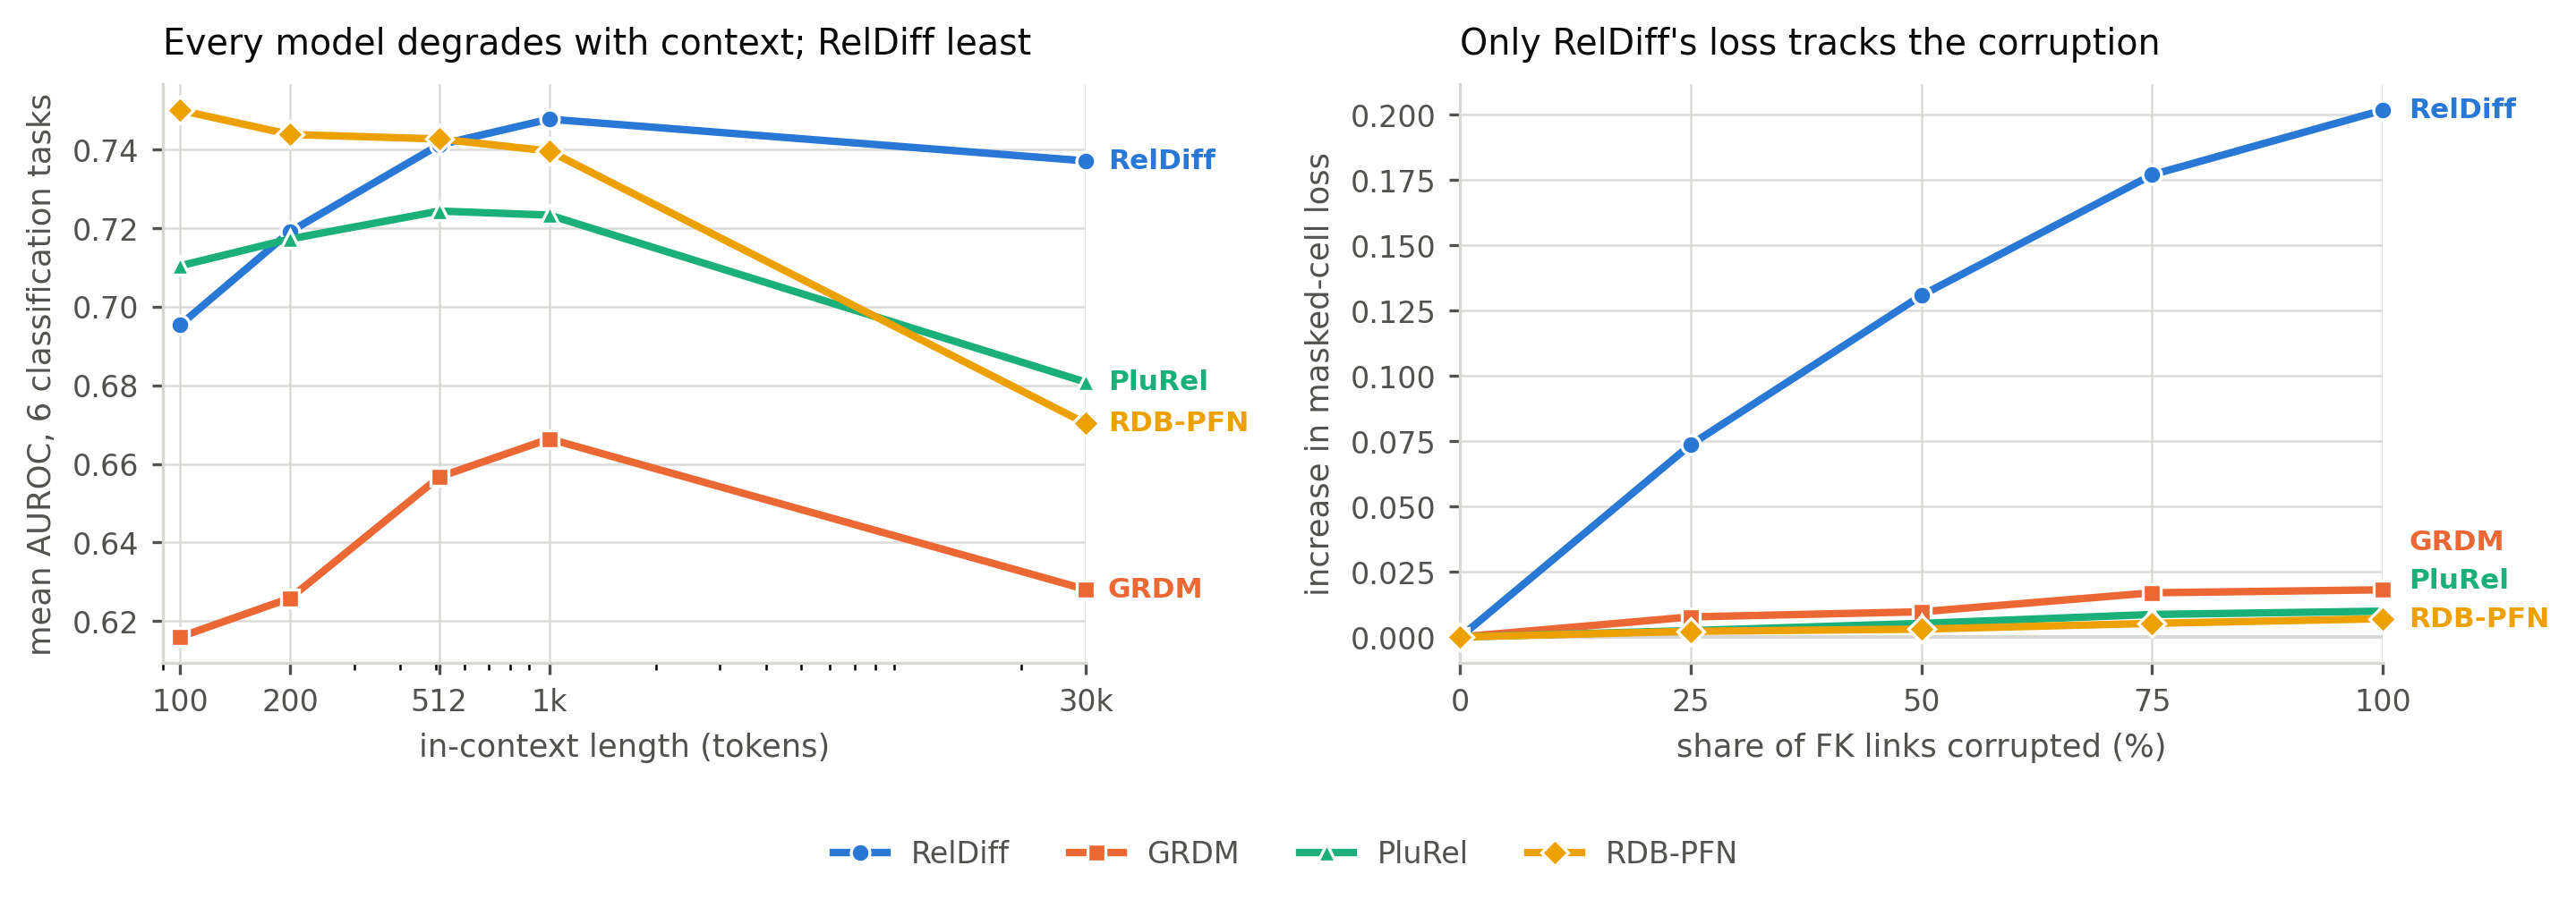
\includegraphics[width=\linewidth]{figs/fig_paper_main.png}
\caption{Left: mean AUROC over the six classification tasks against in-context length. The
30k points for the two \texttt{rel-stack} tasks are our $n{=}2048$ rescoring; at the original
$n{=}256$ they carried only six and ten positive examples. Every model degrades with context
and RelDiff degrades least, by a factor of three or more. Right: masked-cell loss as a graded
fraction of FK links is corrupted. RelDiff's loss tracks the corruption monotonically at
$11$--$29\times$ the slope of the others, which are flat.}
\label{fig:main}
\end{figure}

\begin{table}[t]
\caption{X1: the exact downstream benchmark, rerun under mechanistic ablation, on RelDiff's largest win (\texttt{rel-stack} user-engagement). Ablating exactly the mechanism identified by E1/E5/E7 collapses RelDiff to the pooling models' level; PluRel/RDB-PFN are unaffected by either intervention. All rows use $n{=}2048$ ($\approx$60 positives per cell); the 30k rows were rescored at this sample size after we found the original $n{=}256$ estimates unstable. RelDiff is the only model that moves: corrupting FK structure costs it 0.286 AUROC at 30k, dropping it below the level the structure-blind models reach untouched. PluRel and RDB-PFN are indifferent to both interventions everywhere ($|\Delta| \leq 0.017$), as a bag-of-rows computation should be. GRDM is the informative exception: FK corruption \emph{improves} it by 0.102, the misleading-priors effect that also appears in E7's per-database signs.}
\label{tab:x1}
\centering
\small
\begin{tabular}{llccccc}
\toprule
Ctx & Model & Intact & FK shuffled & Nbr zeroed & $\Delta_{\text{FK}}$ & $\Delta_{\text{nbr}}$ \\
\midrule
30{,}000 & RelDiff  & \textbf{0.865} & \textbf{0.579} & \textbf{0.624} & \textbf{$-$0.286} & \textbf{$-$0.241} \\
30{,}000 & PluRel   & 0.652 & 0.650 & 0.636 & $-$0.003 & $-$0.017 \\
30{,}000 & RDB-PFN  & 0.642 & 0.643 & 0.634 & +0.001 & $-$0.008 \\
30{,}000 & GRDM     & 0.520 & 0.622 & 0.537 & \emph{+0.102} & +0.018 \\
1{,}024  & RelDiff  & 0.847 & 0.718 & 0.728 & $-$0.129 & $-$0.119 \\
1{,}024  & PluRel   & 0.708 & 0.701 & 0.697 & $-$0.007 & $-$0.011 \\
1{,}024  & RDB-PFN  & 0.691 & 0.694 & 0.687 & +0.003 & $-$0.004 \\
1{,}024  & GRDM     & 0.609 & 0.618 & 0.622 & +0.009 & +0.013 \\
\bottomrule
\end{tabular}
\end{table}

Table~\ref{tab:x1} confirms predictions (1)--(3). FK corruption erases RelDiff's engagement advantage at both context lengths, and at 30k it costs 0.286 AUROC --- dropping RelDiff from 0.865 to 0.579, below the 0.642--0.652 the structure-blind models reach with no intervention at all. Long context without the relational mechanism is not merely less useful; it is worse than a shorter context, because pooling over more neighbours adds variance and no signal. PluRel and RDB-PFN are unmoved by either intervention at either length ($|\Delta| \leq 0.017$), which is what a within-row computation predicts. Prediction (4) is refuted in its specific location --- \texttt{rel-arxiv} paper-citation shows only mild, ordinary reliance --- but the phenomenon it anticipated appears twice elsewhere, and in the stronger form: on \texttt{rel-ratebeer} user-churn FK-shuffling improves both structure-using models ($+0.061$, $+0.064$), and on \texttt{rel-stack} user-engagement at 30k it improves GRDM by $+0.102$. Where a model's relational priors fit the task the mechanism produces its wins; where they misfit, the same mechanism produces its losses, and removing it helps.

Taken together, this is a causal double confirmation: the pretraining corpus determines a checkable mechanism (E1/E4/E5/E7), and surgically removing that mechanism --- and only that mechanism, holding the model otherwise fixed --- reproduces the corresponding change in downstream capability, including its failure mode. The generator did not just correlate with a better benchmark score; it built the specific computation the benchmark score depends on.

\section{Related work}

RFM architectures differ in how they model cross-table interaction: message passing \cite{rdl,relgnn,griffin} vs.\ relational attention \cite{relgt,kumorfm,rt}. We build on the RT because its factored attention streams make attribution to a specific computational channel possible, which a message-passing update does not as directly expose. Generators split into reference-conditioned families that regenerate a real schema and FK graph \cite{reldiff,grdm} and reference-free families that sample both from scratch \cite{plurel,rdbpfn}. Prior comparisons rank them by benchmark transfer; we take that ranking as a starting point and ask what mechanism produces it, using linear CKA \cite{cka} for functional rather than weight-level comparison and input/activation ablation for causal validation.

\section{Discussion and limitations}

Our central claim is methodological: benchmark rankings of synthetic-data generators can be decomposed into a checkable mechanism, and that mechanism can be causally validated by ablating exactly what the diagnostics point to, rather than by ablating the generator's identity (retraining from scratch). This is attractive for practitioners choosing or designing a generator for RFM pretraining, because the weight-space diagnostic (E1) is available in minutes on a CPU, before any expensive downstream evaluation, and the ablation protocol (E7/X1) reuses the pretraining objective rather than requiring a new benchmark.

The main limitations are scope and scale. We study one architecture (RT) and one pretraining objective (masked-cell reconstruction); the extent to which weight-stream separation transfers to message-passing RFMs is untested. Each generator arm is a single pretraining run at a short (3.5-hour) step budget shared across arms, so we report the \emph{direction} of weight-space specialization rather than claiming the absolute magnitudes would hold at production-scale pretraining; the CKA and behavioral results (Sec.~\ref{sec:mech}--\ref{sec:bridge}), being measured directly on the trained checkpoints, are not subject to this caveat. Finally, reference-conditioning is neither necessary nor sufficient in isolation: GRDM uses real references yet its relational computation does not transfer beyond its reference schemas. What matters is whether a generator's construction makes cross-table structure predictively necessary (Sec.~\ref{sec:corpus}), which a reference-free generator could in principle also achieve.

\section{Conclusion}

Benchmark comparisons of synthetic-data generators answer \emph{which} is better, not \emph{why}. We show the question is answerable end to end: the property that matters is measurable in the corpus before any model exists, it leaves a predictable imprint in weight space, and ablating the mechanism it builds removes the benchmark advantage it explains. We hope this recipe --- corpus measurement, checkpoint diagnostics, causal ablation --- generalizes to attributing other foundation-model capabilities to checkable properties of their pretraining data.

\begin{ack}
Omitted for anonymous review.
\end{ack}

{\small
\begin{thebibliography}{99}

\bibitem{rdl} Fey, M., Hu, W., Huang, K., Lenssen, J.E., Ranjan, R., Robinson, J., Ying, R., You, J., Leskovec, J.\ (2024) Position: Relational Deep Learning, Graph Representation Learning on Relational Databases. \emph{ICML}.

\bibitem{relbench} Robinson, J., Ranjan, R., Hu, W., et al.\ (2024) RelBench: A Benchmark for Deep Learning on Relational Databases. \emph{NeurIPS Datasets and Benchmarks}.

\bibitem{relgnn} Chen, T., Kanatsoulis, C., Leskovec, J.\ (2025) RelGNN: Composite Message Passing for Relational Deep Learning. \emph{ICML}.

\bibitem{relgt} Dwivedi, V.P., Jaladi, S., Shen, Y., Lopez, F., Kanatsoulis, C., Puri, R., Fey, M., Leskovec, J.\ (2026) Relational Graph Transformers. \emph{ICLR}.

\bibitem{griffin} Wang, Y., Wang, X., Gan, Q., Yang, Y., Wipf, D., Zhang, Z.\ (2025) Griffin: Towards a Graph-Centric Relational Foundation Model. \emph{ICML}.

\bibitem{kumorfm} Fey, M., Kocijan, V., Lopez, F., Lenssen, J.E., Leskovec, J.\ (2025) KumoRFM: A Relational Foundation Model for In-Context Learning on Enterprise Data. Technical report, Kumo.ai.

\bibitem{rt} Ranjan, R., Hudovernik, V., Znidar, M., Kanatsoulis, C., Upendra, A., Mohammadi, S., Meyer, R., Palczewski, J., Guestrin, C., Leskovec, J.\ (2026) Relational Transformer: Toward Zero-Shot Foundation Models for Relational Data. \emph{ICLR}.

\bibitem{reldiff} Hudovernik, V., Xu, M., Shi, K., \v{S}ubelj, L., Ermon, S., \v{S}trumbelj, E., Leskovec, J.\ (2025) RelDiff: Relational Data Generative Modeling with Graph-Based Diffusion Models. arXiv:2506.00710.

\bibitem{plurel} Anonymous.\ (2026) PluRel: Synthetic Data Unlocks Scaling Laws for Relational Foundation Models. arXiv:2602.04029.

\bibitem{grdm} Anonymous.\ Graph-Conditional Relational Diffusion Models for Relational Database Synthesis. Under review.

\bibitem{rdbpfn} Anonymous.\ (2026) Relational In-Context Learning via Synthetic Pre-training with Structural Prior. arXiv:2603.03805.

\bibitem{cka} Kornblith, S., Norouzi, M., Lee, H., Hinton, G.\ (2019) Similarity of Neural Network Representations Revisited. \emph{ICML}.

\bibitem{minilm} Wang, W., Wei, F., Dong, L., Bao, H., Yang, N., Zhou, M.\ (2020) MiniLM: Deep Self-Attention Distillation for Task-Agnostic Compression of Pre-Trained Transformers. \emph{NeurIPS}.

\bibitem{hanley} Hanley, J.A., McNeil, B.J.\ (1982) The meaning and use of the area under a receiver operating characteristic (ROC) curve. \emph{Radiology} 143(1):29--36.

\end{thebibliography}
}

\appendix
\section{Supporting figures}
\label{app:figs}

\begin{figure}[h]
\centering
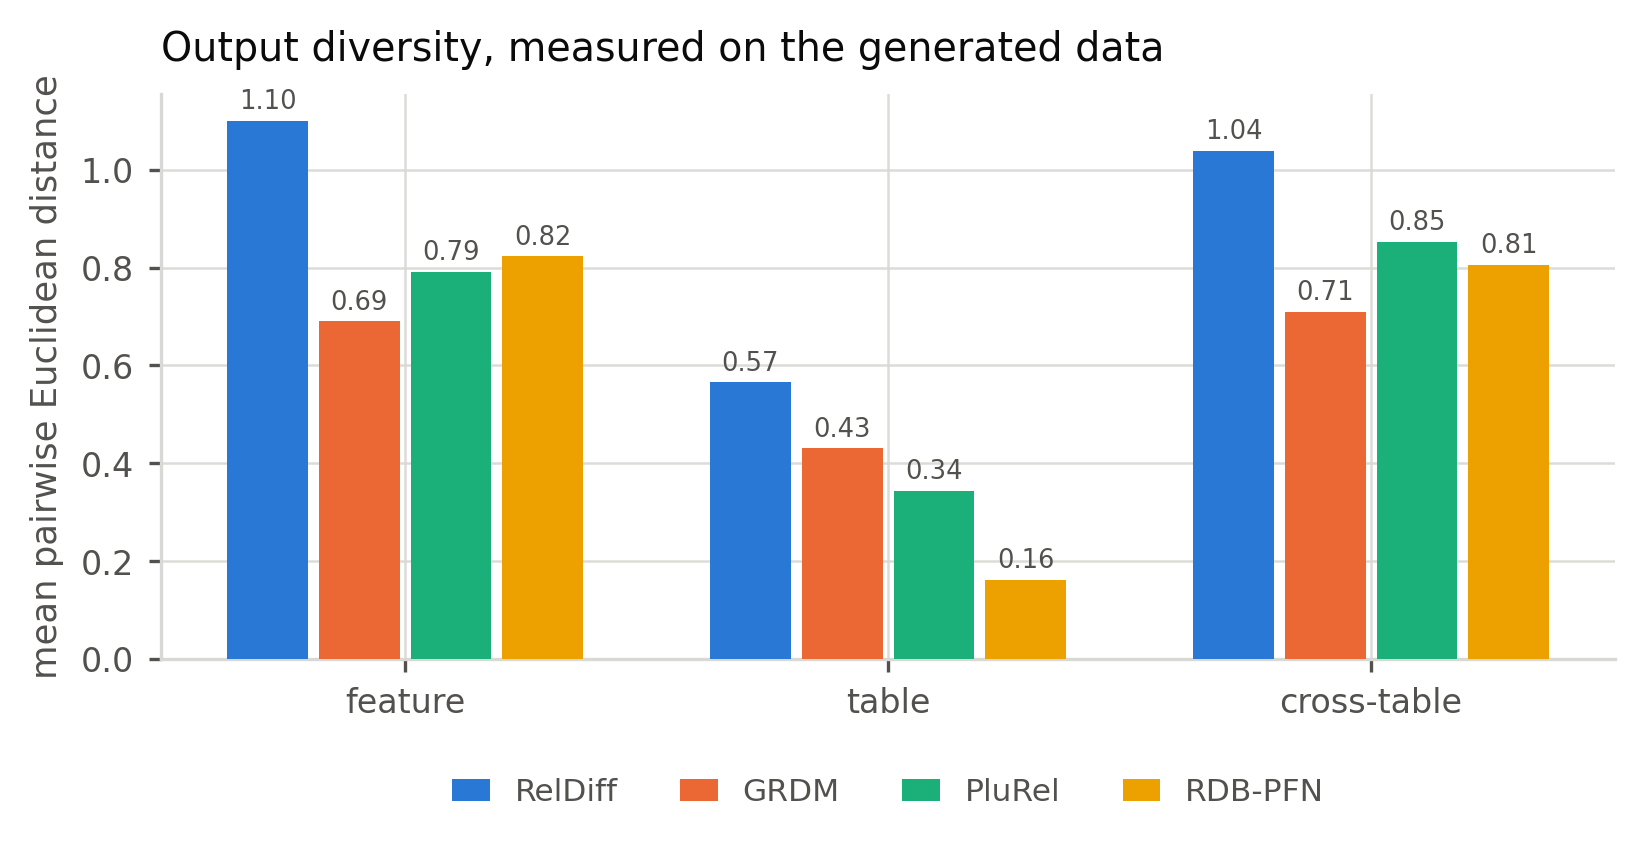
\includegraphics[width=0.70\linewidth]{figs/fig_diversity.png}
\caption{Output diversity of each generator, computed directly from the generated databases
rather than through any model's representation. RelDiff leads on all three axes, but the
ranking of the other three does not track mechanism formation: PluRel exceeds GRDM on
cross-table diversity yet learns no usable relational computation.}
\end{figure}

\begin{figure}[h]
\centering
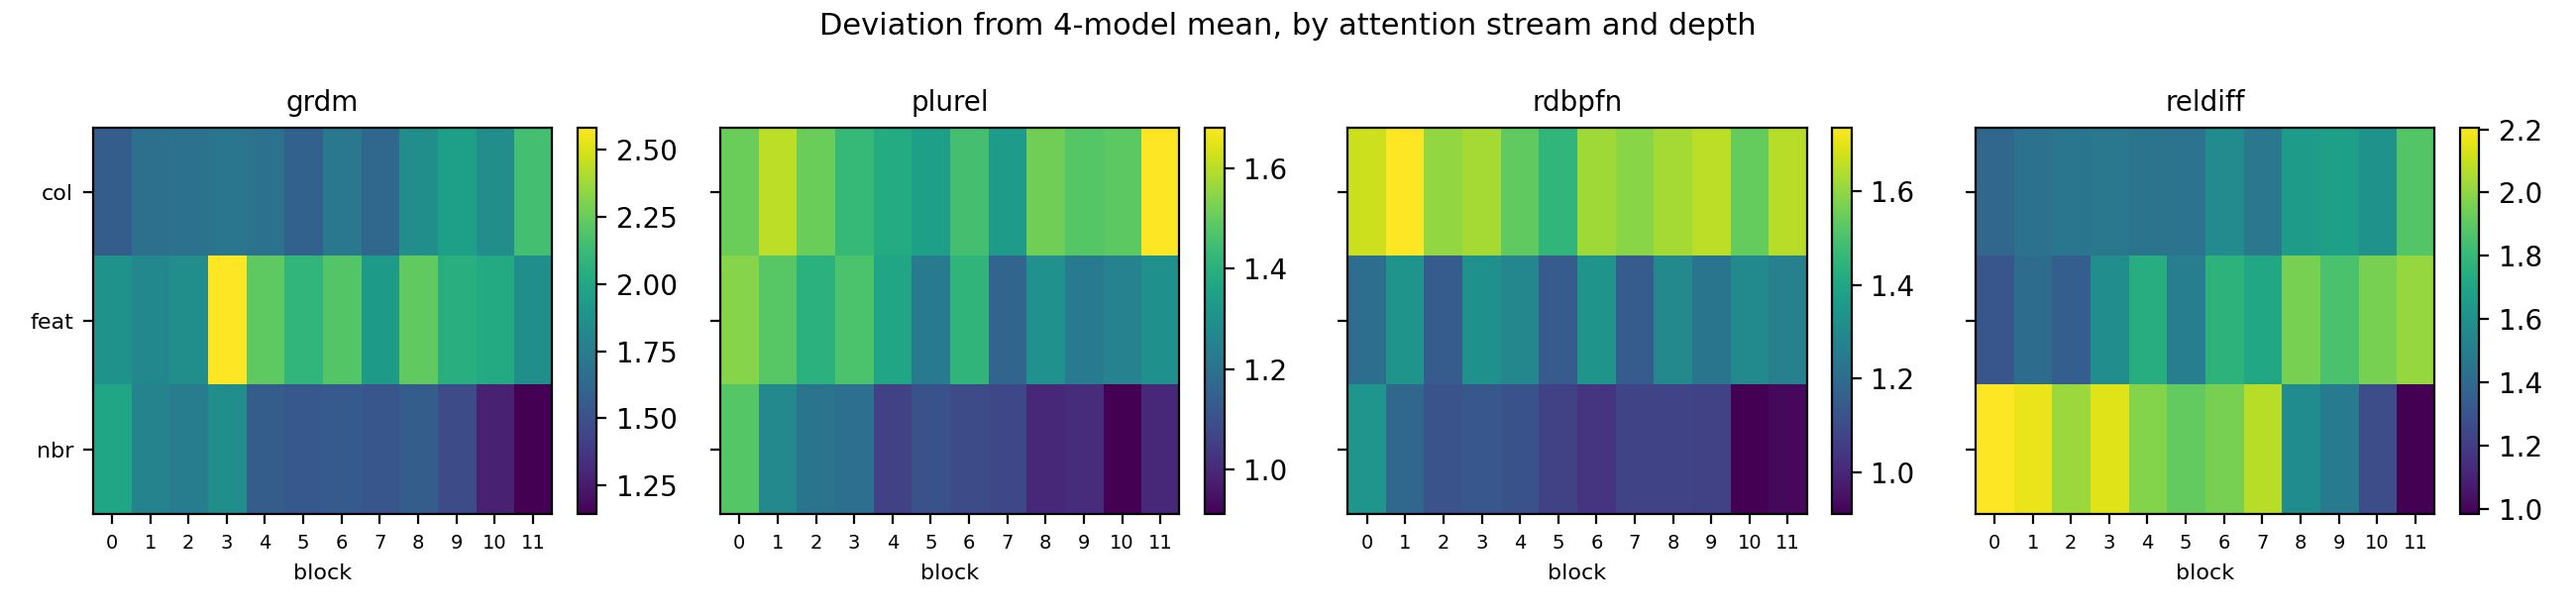
\includegraphics[width=\linewidth]{figs/fig_e1_stream_depth.png}
\caption{E1: deviation from the four-model mean by attention stream and depth. RelDiff is the
only arm whose deviation peaks in \texttt{nbr}; GRDM's peaks in \texttt{feat}.}
\end{figure}

\begin{figure}[h]
\centering
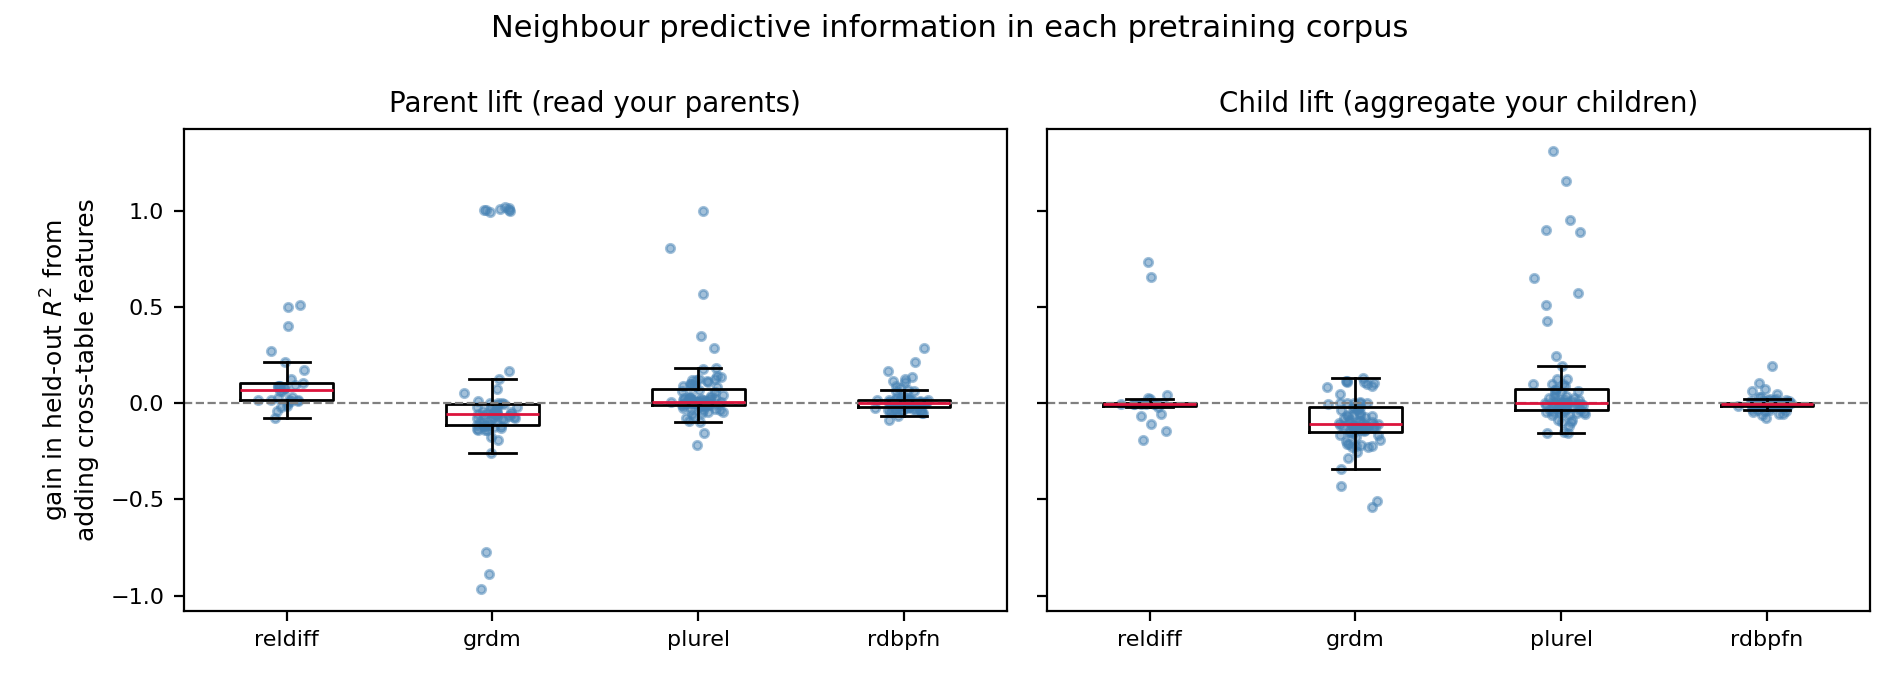
\includegraphics[width=0.78\linewidth]{figs/fig_e2_lift.png}
\caption{Neighbour predictive information per corpus (Sec.~\ref{sec:corpus}). Each point is one
target column; the gain is from adding cross-table features to a within-row baseline.}
\end{figure}

\newpage
\section*{NeurIPS Paper Checklist}

\begin{enumerate}

\item {\bf Claims}
    \item[] Question: Do the main claims made in the abstract and introduction accurately reflect the paper's contributions and scope?
    \item[] Answer: \answerYes{}
    \item[] Justification: The abstract and Sec.~\ref{sec:intro} state exactly the three contributions reported in Sec.~\ref{sec:corpus}--\ref{sec:bridge}: a model-free measurement of neighbour predictive information in the corpora, a weight-space diagnostic, and its causal validation via ablation; we do not claim generalization beyond the single architecture and objective studied (see Limitations).

\item {\bf Limitations}
    \item[] Question: Does the paper discuss the limitations of the work performed by the authors?
    \item[] Answer: \answerYes{}
    \item[] Justification: Section 7 (Discussion and limitations) discusses the single-architecture/single-objective scope, the single pretraining run per generator arm at a short shared step budget, and that reference-conditioning is neither necessary nor sufficient for mechanism formation.

\item {\bf Theory assumptions and proofs}
    \item[] Question: For each theoretical result, does the paper provide the full set of assumptions and a complete (and correct) proof?
    \item[] Answer: \answerNA{}
    \item[] Justification: The paper is purely empirical/mechanistic; it contains no theorems or formal proofs.

\item {\bf Experimental result reproducibility}
    \item[] Question: Does the paper fully disclose all the information needed to reproduce the main experimental results of the paper to the extent that it affects the main claims and/or conclusions of the paper (regardless of whether the code and data are provided or not)?
    \item[] Answer: \answerYes{}
    \item[] Justification: Sec.~\ref{sec:setup} specifies the shared architecture, initialization, step budget, and objective across the four checkpoints; Sec.~\ref{sec:mech}--\ref{sec:bridge} specify the exact probe/ablation protocols (corruption types, probe databases, context lengths, and the causal-ablation predictions registered before running X1) needed to reproduce each table.

\item {\bf Open access to data and code}
    \item[] Question: Does the paper provide open access to the data and code, with sufficient instructions to faithfully reproduce the main experimental results, as described in supplemental material?
    \item[] Answer: \answerNo{}
    \item[] Justification: The four pretraining corpora, checkpoints, and analysis code are being prepared for a public release accompanying the camera-ready version and are not yet hosted at an anonymized URL at submission time.

\item {\bf Experimental setting/details}
    \item[] Question: Does the paper specify all the training and test details (e.g., data splits, hyperparameters, how they were chosen, type of optimizer) necessary to understand the results?
    \item[] Answer: \answerYes{}
    \item[] Justification: Sec.~\ref{sec:setup} specifies the architecture, encoders, and shared pretraining protocol; Sec.~\ref{sec:mech} specifies the held-out, out-of-reference-set evaluation databases and probe-batch protocol used for every mechanistic measurement.

\item {\bf Experiment statistical significance}
    \item[] Answer: \answerNo{}
    \item[] Justification: Each generator arm corresponds to a single pretraining run (shared compute budget across four arms), so we do not report error bars across seeds; we mitigate this by cross-validating each finding across four independent diagnostics (E1, E4, E5, E7) and a causal ablation (X1) rather than relying on any single point estimate, and we discuss this as a limitation in Sec.~7.

\item {\bf Experiments compute resources}
    \item[] Question: For each experiment, does the paper provide sufficient information on the computer resources (type of compute workers, memory, time of execution) needed to reproduce the experiments?
    \item[] Answer: \answerYes{}
    \item[] Justification: Sec.~\ref{sec:mech} notes that the weight-space diagnostic (E1) runs in minutes on a single CPU with no dataloader, while the representational, attention, and ablation probes (E4, E5, E7) and the causal-bridge benchmark (X1) require a GPU box for activation extraction and inference; Sec.~7 states the shared 3.5-hour pretraining budget per arm.

\item {\bf Code of ethics}
    \item[] Question: Does the research conducted in the paper conform, in every respect, with the NeurIPS Code of Ethics?
    \item[] Answer: \answerYes{}
    \item[] Justification: The work analyzes model checkpoints and synthetic/public benchmark data; it involves no human subjects, private data, or crowdsourcing.

\item {\bf Broader impacts}
    \item[] Question: Does the paper discuss both potential positive societal impacts and negative societal impacts of the work performed?
    \item[] Answer: \answerYes{}
    \item[] Justification: Sec.~7 frames the positive impact (a cheap, pre-deployment diagnostic for whether a synthetic-data pipeline taught a foundation model a genuine, transferable skill rather than a benchmark-specific artifact); we are not aware of a direct negative-impact pathway specific to this attribution methodology beyond those already inherent to relational foundation models generally.

\item {\bf Safeguards}
    \item[] Question: Does the paper describe safeguards that have been put in place for responsible release of data or models that have a high risk for misuse?
    \item[] Answer: \answerNA{}
    \item[] Justification: The released checkpoints are small (19.2M-parameter) research artifacts trained on synthetic and public benchmark relational data; they pose no high-risk dual-use profile requiring gated release.

\item {\bf Licenses for existing assets}
    \item[] Question: Are the creators or original owners of assets used in the paper properly credited and are the license and terms of use explicitly mentioned and properly respected?
    \item[] Answer: \answerYes{}
    \item[] Justification: We cite the RelBench benchmark and the RT architecture and each of the four generators (RelDiff, GRDM, PluRel, RDB-PFN) by their source papers/repositories in the References, and use each only under its stated license and terms.

\item {\bf New assets}
    \item[] Question: Are new assets introduced in the paper well documented and is the documentation provided alongside the assets?
    \item[] Answer: \answerYes{}
    \item[] Justification: The four pretrained RT checkpoints and the mechanistic-analysis probes (E1--E7, X1--X2) are new artifacts of this work; Sec.~\ref{sec:setup}--\ref{sec:bridge} document their construction and intended use, and full documentation will accompany the code/checkpoint release referenced in item 5.

\item {\bf Crowdsourcing and research with human subjects}
    \item[] Answer: \answerNA{}
    \item[] Justification: The paper does not involve crowdsourcing or human subjects.

\item {\bf Institutional review board (IRB) approvals or equivalent for research with human subjects}
    \item[] Answer: \answerNA{}
    \item[] Justification: The paper does not involve human subjects research.

\item {\bf Declaration of LLM usage}
    \item[] Question: Does the paper describe the usage of LLMs if it is an important, original, or non-standard component of the core methods in this research?
    \item[] Answer: \answerNA{}
    \item[] Justification: The only LLM-adjacent component is a fixed, off-the-shelf MiniLM text encoder inherited unmodified from the pre-existing RT architecture (Sec.~\ref{sec:setup}); it is not a novel or original component of this paper's core method, which is the mechanistic attribution analysis itself.

\end{enumerate}


\end{document}
